\documentclass[a4paper,12pt]{article}
\usepackage[indonesian]{babel}
\usepackage{graphicx}
\usepackage{multirow}
\usepackage{enumitem}
\usepackage{listings}
\usepackage{wrapfig}
\usepackage[T1]{fontenc}
\usepackage{inconsolata}
\usepackage{lipsum}
\usepackage{adjustbox}


\usepackage{color}
\usepackage[table]{xcolor}
\definecolor{mygreen}{rgb}{0,0.6,0}
\definecolor{mygray}{rgb}{0.5,0.5,0.5}
\definecolor{mymauve}{rgb}{0.58,0,0.82}
\lstset{%
    language=java,
    showstringspaces=false,          % Prevent tex replacing space to bracket in code
    frame=single,                    % Set frame around code
    backgroundcolor=\color{white},   % choose the background color
    basicstyle=\footnotesize,        % size of fonts used for the code
    breaklines=true,                 % automatic line breaking only at whitespace
    captionpos=b,                    % sets the caption-position to bottom
    commentstyle=\color{mygreen},    % comment style
    keywordstyle=\color{blue},       % keyword style
    stringstyle=\color{mymauve},     % string literal style
    numbers=left,
}

\graphicspath{ {./img/} }
\begin{document}
\title{ {\Large Laporan Praktikum}\\ Algoritma dan Pemrograman Lanjut\\{\Large Pertemuan 14}}

\author{Aldzikri Dwijayanto Prathama
    \\195410189
    \\Informatika}
\makeatletter
\begin{titlepage}
    \begin{center}
        {\huge \bfseries \@title}\\[14ex]
        
\includegraphics[scale=.8]{logo}\\[4ex]
        {\large \@author}\\[12ex]
        {\large \bfseries {SEKOLAH TINGGI MANAJEMEN INFORMATIKA DAN KOMPUTER
            AKAKOM YOGYAKARTA}}
    \end{center}


%{\large \@date}
\end{titlepage}
\makeatother
%\maketitle
\newpage
\tableofcontents
\newpage

\section{Tujuan}
Mahasiswa dapat melakukan pencarian data dengan metode linear search dan
mengimplementasikannya dalam program.
\section{Teori}
Searching (pencarian) adalah aplikasi komputer yang sangat penting. Dalam pencarian,hal yang paling penting adalah
adanya kunci pencarian. Searching adalah algoritma untukmencari data yang berada pada suatu kumpulan data tertentu.
Pencarian terhadap data, bisamerupakan data yang sudah terurut maupun yang belum terurut.

\newpage

\section{Pembahasan}
\subsection{Praktik}
\subsubsection{Praktik 1}
\begin{lstlisting}
import java.util.Scanner;

public class Larik9 {
    public static void main(String args[]) {
        Scanner input = new Scanner(System.in);
        int i, x;
        boolean ketemu;
        int data[] = { 12, 20, 14, 9, 34 };
        System.out.print("Masukan Data yang dicari = ");
        x = input.nextInt();
        ketemu = false;
        for (i = 0; i < 5; i++) {
            if (data[i] == x) {
                ketemu = !ketemu;
                break;
            }
        }
        if (ketemu)
            System.out.println("Data tersebut ada pada posisi ke-" + (i + 1));
        else
            System.out.println("Data tidak ketemu !");
    }
}
\end{lstlisting}

\textbf{Pencarian Linear\\}
Pencarian linear adalah sebuah algoritme pencarian, juga dikenal sebagai pencarian sekuensial, yang cocok untuk mencari
sebuah nilai tertentu pada sebuah himpunan data. 
Algoritme ini beroperasi dengan memeriksa setiap elemen dari sebuah list sampai sebuah kecocokan ditemukan. Pencarian
linear bekerja dalam O(n). Jika data terdistribusi secara acak, rata-rata ada n/2 pembandingan akan dilakukan. Kasus
terbaik adalah ketika nilai yang dicari adalah elemen pertama dari list, kasus ini hanya memerlukan 1 pembandingan.
Kasus terburuk adalah ketika nilai yang dicari tidak ada dalam list, yang memerlukan n pembadingan.

\begin{center}
    
\includegraphics[scale=1]{1.png} 
\end{center}

\subsection{Latihan}
\begin{lstlisting}
import java.util.Scanner;

public class LinearSearchR {
    static int data[] = { 12, 20, 14, 9, 34 };

    public static int LinearSearch(int kunci, int indeksAwal) {
        if (kunci == data[indeksAwal])
            return indeksAwal;
        if (indeksAwal + 1 < data.length)
            return LinearSearch(kunci, indeksAwal + 1);
        return -1;
    }

    public static void main(String args[]) {

        Scanner input = new Scanner(System.in);
        int i, x;
        System.out.print("Masukan Data yang dicari = *");
        x = input.nextInt();
        i = LinearSearch(x, 0);
        if (i != -1)
            System.out.println("Data tersebut ada pada posisi ke-" + i);
        else
            System.out.println("Data tidak ketemu !");
    }
}
\end{lstlisting}

Pencarian linear adalah sebuah algoritme pencarian, juga dikenal sebagai pencarian sekuensial, yang cocok untuk mencari
sebuah nilai tertentu pada sebuah himpunan data. 
Algoritme ini beroperasi dengan memeriksa setiap elemen dari sebuah list sampai sebuah kecocokan ditemukan. Pencarian
linear bekerja dalam O(n). Jika data terdistribusi secara acak, rata-rata ada n/2 pembandingan akan dilakukan. Kasus
terbaik adalah ketika nilai yang dicari adalah elemen pertama dari list, kasus ini hanya memerlukan 1 pembandingan.
Kasus terburuk adalah ketika nilai yang dicari tidak ada dalam list, yang memerlukan n pembadingan.\\

Algoritma pada program di atas adalah sebagai berikut:
\begin{enumerate}
    \item Program mulai mencari dari elemen array paling kiri, dan satu persatu membandingkan x dengan setiap elemen
        array.
    \item Jika x sesuai dengan salah satu elemen, maka method akan mengembalikan index.
    \item jika x tidak cocok dengan semua elemen, maka method akan mengembalikan nilai -1.
\end{enumerate}
\begin{center}
    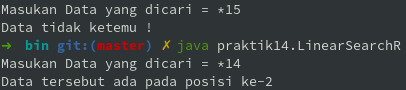
\includegraphics[scale=1]{2.png} 
\end{center}

\newpage

\subsection{Tugas}
\begin{lstlisting}
import java.util.List;
import java.util.Arrays;
import java.util.Collections;
import java.util.ArrayList;

public class BinarySearchTest {
    public static void main(String[] args) {
        // create an ArrayListe String > from the cantents of colors array
        String[] colors = { "red", "white", "blue", "black", "yellow", "purple", "tan", "pink" };
        List<String> list = new ArrayList<String>(Arrays.asList(colors));

        Collections.sort(list); // sort the Arcaylist
        System.out.printf("Sorted ArrayList: ss\n", list);

        // search 1ist for various values
        printSearchResults(list, colors[3]); // first item
        printSearchResults(list, colors[0]); // middle item
        printSearchResults(list, colors[7]); // last item
        printSearchResults(list, "aqua"); // below lowest
        printSearchResults(list, "gray"); // does not exist
        printSearchResults(list, "teal"); // does not exist

    }// end main

    // perforn search and display result
    private static void printSearchResults(List<String> list, String key) {

        int result = 0;

        System.out.printf("\nSearching for: %s\n", key);
        result = Collections.binarySearch(list, key);

        if (result >= 0)
            System.out.printf("Found at index %d\n", result);
        else
            System.out.printf("Not Found (%d)\n", result);
    } // end metnoa printsearchResults
} // end class BinarysearchTest
\end{lstlisting}
Pencarian Biner (\textit{Binary Search}) adalah pencarian data secara eliminasi biner berulang/terus-menerus. Maksudnya
adalah pada saat pencarian data, 1 kelompok data yang sudah urut dibagi menjadi 2 subkelompok. Lalu salah satu
subkelompok dieliminasi, sehingga ruang lingkup pencarian data menjadi lebih sedikit. Kemudian subkelompok yang tersisa
dibagi lagi menjadi 2 subkelompok lagi, demikian dilakukan secara berulang-ulang.

\newpage

\section{Kesimpulan}
Setelah praktik ini mahasiswa dapat melakukan pencarian data dengan metode linear search dan
mengimplementasikannya dalam program.
\end{document}
